\subsection{Image of a promeasure}

Let E and \(E_{1}\) be two locally convex spaces, and u a continuous linear mapping of E into \(E_{1}\) . For every \(V_{1} \in \mathcal{F}(E_{1})\) , the subspace \(V = \overline{u}^{1}(V_{1})\) of E belongs to \(\mathcal{F}(E)\) , and u defines, by passage to the quotients, a linear mapping \(u_{V_{1}}\) of E/V into \(E_{1}/V_{1}\) . Let \(V_{1}\) and \(W_{1}\) in \(\mathcal{F}(E_{1})\) be such that \(V_{1} \supset W_{1}\) ; set \(V = \overline{u}^{1}(V_{1})\) and \(W = \overline{u}^{1}(W_{1})\) . We have \(V \supset W\) , and a commutative diagram

\pandocbounded{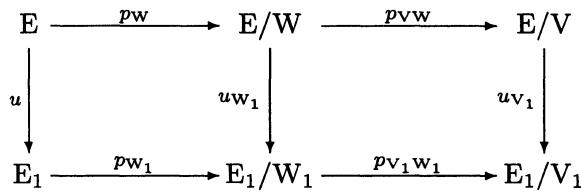
\includegraphics[keepaspectratio]{images/part002_2ec1bcbe.jpg}}

Now let \(\mu = (\mu_{\mathrm{V}})_{\mathrm{V}\in \mathcal{F}(\mathrm{E})}\) be a promeasure on \(\mathbf{E}\) . For every \(\mathrm{V}_1\in \mathcal{F}(\mathrm{E}_1)\) , set

\[
\nu_ {\mathrm{V} _ {1}} = u _ {\mathrm{V} _ {1}} \left(\mu_ {u ^ {- 1} \left(\mathrm{V} _ {1}\right)}\right).\tag{1}
\]

The commutativity of the preceding diagram shows that the family \(\nu = (\nu_{\mathrm{V}_1})_{\mathrm{V}_1 \in \mathcal{F}(\mathrm{E}_1)}\) is a promeasure on \(\mathbf{E}_1\) . We say that \(\nu\) is the image of \(\mu\) under \(u\) , and denote it by \(u(\mu)\) .

Let \(\lambda\) be a bounded measure on E, and \(u(\lambda)\) the measure on \(E_{1}\) that is the image of \(\lambda\) under u. If the promeasure \(\mu\) is associated with \(\lambda\) , then the promeasure \(u(\mu)\) is associated with \(u(\lambda)\) . This follows from the commutativity of the preceding diagram.

Let \(V \in \mathcal{F}(E)\) . It is immediate that the image promeasure on \(E/V\) of the promeasure \(\mu\) under the canonical mapping \(p_V: E \to E/V\) is associated with the measure \(\mu_V\) .

Let \(u_{1}\) be a continuous linear mapping of \(E_{1}\) into a locally convex space \(E_{2}\) . One establishes without difficulty the relation

\[
(u _ {1} \circ u) (\mu) = u _ {1} (u (\mu))
\]

(transitivity of the images of promeasures).

